\documentclass[../../../../doc.tex]{subfiles}

\begin{document}
\subsection{Algorytm A*}

Działa jak BFS z wykorzystaniem zamiast zwykłej kolejki, kolejki prioretytowej która jako prirorytetu używa
sumy heurystyki i dystansu.


Przykład działania algorytmu przedstawia \cref{fig:astar_solve_steps}.

\begin{figure}[H]
\centering
\begin{minipage}[t]{0.48\textwidth}
\centering
          
  \begin{tikzpicture}[scale=0.8]
  \node at (1.5, 0.5){\color{blue}\faIcon{user}};
\fill[gray] (2, 0) rectangle (3, 1);
\fill[gray] (0, 1) rectangle (1, 2);
\fill[gray] (2, 1) rectangle (3, 2);
\fill[gray] (4, 1) rectangle (5, 2);
\fill[gray] (0, 2) rectangle (1, 3);
\fill[gray] (2, 2) rectangle (3, 3);
\fill[gray] (4, 2) rectangle (5, 3);
\node at (4.5, 3.5){\color{blue}\faIcon{home}};
\fill[gray] (0, 4) rectangle (1, 5);
\fill[gray] (1, 4) rectangle (2, 5);
\fill[gray] (3, 4) rectangle (4, 5);
\fill[gray] (4, 4) rectangle (5, 5);
\draw[black] grid (5, 5);
  \end{tikzpicture}
  
          \caption{\centering Dodaj do kolejki węzeł (1,0).}
          \label{fig:astar_solve_steps_start}
\end{minipage}\hfill
\begin{minipage}[t]{0.48\textwidth}
          \centering
          
  \begin{tikzpicture}[scale=0.8]
  \node at (1.5, 0.5){\color{blue}\faIcon{user}};
\fill[gray] (2, 0) rectangle (3, 1);
\fill[gray] (0, 1) rectangle (1, 2);
\fill[gray] (2, 1) rectangle (3, 2);
\fill[gray] (4, 1) rectangle (5, 2);
\fill[gray] (0, 2) rectangle (1, 3);
\fill[gray] (2, 2) rectangle (3, 3);
\fill[gray] (4, 2) rectangle (5, 3);
\node at (4.5, 3.5){\color{blue}\faIcon{home}};
\fill[gray] (0, 4) rectangle (1, 5);
\fill[gray] (1, 4) rectangle (2, 5);
\fill[gray] (3, 4) rectangle (4, 5);
\fill[gray] (4, 4) rectangle (5, 5);
\draw[black] grid (5, 5);
  \end{tikzpicture}
  
          \caption{\centering Rozpatrz pole (1,0).}
\end{minipage}
\end{figure}

\begin{figure}[H]
\centering
\begin{minipage}[t]{0.48\textwidth}
          \centering
          
  \begin{tikzpicture}[scale=0.8]
  \node at (1.5, 0.5){\color{blue}\faIcon{user}};
\fill[gray] (2, 0) rectangle (3, 1);
\fill[gray] (0, 1) rectangle (1, 2);
\node at (1.5, 1.5){\color{purple}\faIcon{hourglass}};
\fill[gray] (2, 1) rectangle (3, 2);
\fill[gray] (4, 1) rectangle (5, 2);
\fill[gray] (0, 2) rectangle (1, 3);
\fill[gray] (2, 2) rectangle (3, 3);
\fill[gray] (4, 2) rectangle (5, 3);
\node at (4.5, 3.5){\color{blue}\faIcon{home}};
\fill[gray] (0, 4) rectangle (1, 5);
\fill[gray] (1, 4) rectangle (2, 5);
\fill[gray] (3, 4) rectangle (4, 5);
\fill[gray] (4, 4) rectangle (5, 5);
\draw[black] grid (5, 5);
  \end{tikzpicture}
  
          \caption{\centering Dodaj do kolejki węzeł (1,1).}
\end{minipage}\hfill
\begin{minipage}[t]{0.48\textwidth}
          \centering
          
  \begin{tikzpicture}[scale=0.8]
  \node at (0.5, 0.5){\color{purple}\faIcon{hourglass}};
\node at (1.5, 0.5){\color{blue}\faIcon{user}};
\fill[gray] (2, 0) rectangle (3, 1);
\fill[gray] (0, 1) rectangle (1, 2);
\node at (1.5, 1.5){\color{purple}\faIcon{hourglass}};
\fill[gray] (2, 1) rectangle (3, 2);
\fill[gray] (4, 1) rectangle (5, 2);
\fill[gray] (0, 2) rectangle (1, 3);
\fill[gray] (2, 2) rectangle (3, 3);
\fill[gray] (4, 2) rectangle (5, 3);
\node at (4.5, 3.5){\color{blue}\faIcon{home}};
\fill[gray] (0, 4) rectangle (1, 5);
\fill[gray] (1, 4) rectangle (2, 5);
\fill[gray] (3, 4) rectangle (4, 5);
\fill[gray] (4, 4) rectangle (5, 5);
\draw[black] grid (5, 5);
  \end{tikzpicture}
  
          \caption{\centering Dodaj do kolejki węzeł (0,0).}
\end{minipage}
\end{figure}

\begin{figure}[H]
\centering
\begin{minipage}[t]{0.48\textwidth}
          \centering
          
  \begin{tikzpicture}[scale=0.8]
  \node at (0.5, 0.5){\color{purple}\faIcon{hourglass}};
\node at (1.5, 0.5){\color{blue}\faIcon{user}};
\fill[gray] (2, 0) rectangle (3, 1);
\fill[gray] (0, 1) rectangle (1, 2);
\node at (1.5, 1.5){\color{orange}\faIcon{arrows-alt}};
\fill[gray] (2, 1) rectangle (3, 2);
\fill[gray] (4, 1) rectangle (5, 2);
\fill[gray] (0, 2) rectangle (1, 3);
\fill[gray] (2, 2) rectangle (3, 3);
\fill[gray] (4, 2) rectangle (5, 3);
\node at (4.5, 3.5){\color{blue}\faIcon{home}};
\fill[gray] (0, 4) rectangle (1, 5);
\fill[gray] (1, 4) rectangle (2, 5);
\fill[gray] (3, 4) rectangle (4, 5);
\fill[gray] (4, 4) rectangle (5, 5);
\draw[black] grid (5, 5);
  \end{tikzpicture}
  
          \caption{\centering Rozpatrz pole (1,1).}
\end{minipage}\hfill
\begin{minipage}[t]{0.48\textwidth}
          \centering
          
  \begin{tikzpicture}[scale=0.8]
  \node at (0.5, 0.5){\color{purple}\faIcon{hourglass}};
\node at (1.5, 0.5){\color{blue}\faIcon{user}};
\fill[gray] (2, 0) rectangle (3, 1);
\fill[gray] (0, 1) rectangle (1, 2);
\node at (1.5, 1.5){\color{orange}\faIcon{arrows-alt}};
\fill[gray] (2, 1) rectangle (3, 2);
\fill[gray] (4, 1) rectangle (5, 2);
\fill[gray] (0, 2) rectangle (1, 3);
\node at (1.5, 2.5){\color{purple}\faIcon{hourglass}};
\fill[gray] (2, 2) rectangle (3, 3);
\fill[gray] (4, 2) rectangle (5, 3);
\node at (4.5, 3.5){\color{blue}\faIcon{home}};
\fill[gray] (0, 4) rectangle (1, 5);
\fill[gray] (1, 4) rectangle (2, 5);
\fill[gray] (3, 4) rectangle (4, 5);
\fill[gray] (4, 4) rectangle (5, 5);
\draw[black] grid (5, 5);
  \end{tikzpicture}
  
          \caption{\centering Dodaj do kolejki węzeł (1,2).}
\end{minipage}
\end{figure}

\begin{figure}[H]
\centering
\begin{minipage}[t]{0.48\textwidth}
          \centering
          
  \begin{tikzpicture}[scale=0.8]
  \node at (0.5, 0.5){\color{purple}\faIcon{hourglass}};
\node at (1.5, 0.5){\color{blue}\faIcon{user}};
\fill[gray] (2, 0) rectangle (3, 1);
\fill[gray] (0, 1) rectangle (1, 2);
\node at (1.5, 1.5){\color{orange}\faIcon{arrows-alt}};
\fill[gray] (2, 1) rectangle (3, 2);
\fill[gray] (4, 1) rectangle (5, 2);
\fill[gray] (0, 2) rectangle (1, 3);
\node at (1.5, 2.5){\color{orange}\faIcon{arrows-alt}};
\fill[gray] (2, 2) rectangle (3, 3);
\fill[gray] (4, 2) rectangle (5, 3);
\node at (4.5, 3.5){\color{blue}\faIcon{home}};
\fill[gray] (0, 4) rectangle (1, 5);
\fill[gray] (1, 4) rectangle (2, 5);
\fill[gray] (3, 4) rectangle (4, 5);
\fill[gray] (4, 4) rectangle (5, 5);
\draw[black] grid (5, 5);
  \end{tikzpicture}
  
          \caption{\centering Rozpatrz pole (1,2).}
\end{minipage}\hfill
\begin{minipage}[t]{0.48\textwidth}
          \centering
          
  \begin{tikzpicture}[scale=0.8]
  \node at (0.5, 0.5){\color{purple}\faIcon{hourglass}};
\node at (1.5, 0.5){\color{blue}\faIcon{user}};
\fill[gray] (2, 0) rectangle (3, 1);
\fill[gray] (0, 1) rectangle (1, 2);
\node at (1.5, 1.5){\color{orange}\faIcon{arrows-alt}};
\fill[gray] (2, 1) rectangle (3, 2);
\fill[gray] (4, 1) rectangle (5, 2);
\fill[gray] (0, 2) rectangle (1, 3);
\node at (1.5, 2.5){\color{orange}\faIcon{arrows-alt}};
\fill[gray] (2, 2) rectangle (3, 3);
\fill[gray] (4, 2) rectangle (5, 3);
\node at (1.5, 3.5){\color{purple}\faIcon{hourglass}};
\node at (4.5, 3.5){\color{blue}\faIcon{home}};
\fill[gray] (0, 4) rectangle (1, 5);
\fill[gray] (1, 4) rectangle (2, 5);
\fill[gray] (3, 4) rectangle (4, 5);
\fill[gray] (4, 4) rectangle (5, 5);
\draw[black] grid (5, 5);
  \end{tikzpicture}
  
          \caption{\centering Dodaj do kolejki węzeł (1,3).}
\end{minipage}
\end{figure}

\begin{figure}[H]
\centering
\begin{minipage}[t]{0.48\textwidth}
          \centering
          
  \begin{tikzpicture}[scale=0.8]
  \node at (0.5, 0.5){\color{purple}\faIcon{hourglass}};
\node at (1.5, 0.5){\color{blue}\faIcon{user}};
\fill[gray] (2, 0) rectangle (3, 1);
\fill[gray] (0, 1) rectangle (1, 2);
\node at (1.5, 1.5){\color{orange}\faIcon{arrows-alt}};
\fill[gray] (2, 1) rectangle (3, 2);
\fill[gray] (4, 1) rectangle (5, 2);
\fill[gray] (0, 2) rectangle (1, 3);
\node at (1.5, 2.5){\color{orange}\faIcon{arrows-alt}};
\fill[gray] (2, 2) rectangle (3, 3);
\fill[gray] (4, 2) rectangle (5, 3);
\node at (1.5, 3.5){\color{orange}\faIcon{arrows-alt}};
\node at (4.5, 3.5){\color{blue}\faIcon{home}};
\fill[gray] (0, 4) rectangle (1, 5);
\fill[gray] (1, 4) rectangle (2, 5);
\fill[gray] (3, 4) rectangle (4, 5);
\fill[gray] (4, 4) rectangle (5, 5);
\draw[black] grid (5, 5);
  \end{tikzpicture}
  
          \caption{\centering Rozpatrz pole (1,3).}
\end{minipage}\hfill
\begin{minipage}[t]{0.48\textwidth}
          \centering
          
  \begin{tikzpicture}[scale=0.8]
  \node at (0.5, 0.5){\color{purple}\faIcon{hourglass}};
\node at (1.5, 0.5){\color{blue}\faIcon{user}};
\fill[gray] (2, 0) rectangle (3, 1);
\fill[gray] (0, 1) rectangle (1, 2);
\node at (1.5, 1.5){\color{orange}\faIcon{arrows-alt}};
\fill[gray] (2, 1) rectangle (3, 2);
\fill[gray] (4, 1) rectangle (5, 2);
\fill[gray] (0, 2) rectangle (1, 3);
\node at (1.5, 2.5){\color{orange}\faIcon{arrows-alt}};
\fill[gray] (2, 2) rectangle (3, 3);
\fill[gray] (4, 2) rectangle (5, 3);
\node at (0.5, 3.5){\color{purple}\faIcon{hourglass}};
\node at (1.5, 3.5){\color{orange}\faIcon{arrows-alt}};
\node at (4.5, 3.5){\color{blue}\faIcon{home}};
\fill[gray] (0, 4) rectangle (1, 5);
\fill[gray] (1, 4) rectangle (2, 5);
\fill[gray] (3, 4) rectangle (4, 5);
\fill[gray] (4, 4) rectangle (5, 5);
\draw[black] grid (5, 5);
  \end{tikzpicture}
  
          \caption{\centering Dodaj do kolejki węzeł (0,3).}
\end{minipage}
\end{figure}

\begin{figure}[H]
\centering
\begin{minipage}[t]{0.48\textwidth}
          \centering
          
  \begin{tikzpicture}[scale=0.8]
  \node at (0.5, 0.5){\color{purple}\faIcon{hourglass}};
\node at (1.5, 0.5){\color{blue}\faIcon{user}};
\fill[gray] (2, 0) rectangle (3, 1);
\fill[gray] (0, 1) rectangle (1, 2);
\node at (1.5, 1.5){\color{orange}\faIcon{arrows-alt}};
\fill[gray] (2, 1) rectangle (3, 2);
\fill[gray] (4, 1) rectangle (5, 2);
\fill[gray] (0, 2) rectangle (1, 3);
\node at (1.5, 2.5){\color{orange}\faIcon{arrows-alt}};
\fill[gray] (2, 2) rectangle (3, 3);
\fill[gray] (4, 2) rectangle (5, 3);
\node at (0.5, 3.5){\color{purple}\faIcon{hourglass}};
\node at (1.5, 3.5){\color{orange}\faIcon{arrows-alt}};
\node at (2.5, 3.5){\color{purple}\faIcon{hourglass}};
\node at (4.5, 3.5){\color{blue}\faIcon{home}};
\fill[gray] (0, 4) rectangle (1, 5);
\fill[gray] (1, 4) rectangle (2, 5);
\fill[gray] (3, 4) rectangle (4, 5);
\fill[gray] (4, 4) rectangle (5, 5);
\draw[black] grid (5, 5);
  \end{tikzpicture}
  
          \caption{\centering Dodaj do kolejki węzeł (2,3).}
\end{minipage}\hfill
\begin{minipage}[t]{0.48\textwidth}
          \centering
          
  \begin{tikzpicture}[scale=0.8]
  \node at (0.5, 0.5){\color{purple}\faIcon{hourglass}};
\node at (1.5, 0.5){\color{blue}\faIcon{user}};
\fill[gray] (2, 0) rectangle (3, 1);
\fill[gray] (0, 1) rectangle (1, 2);
\node at (1.5, 1.5){\color{orange}\faIcon{arrows-alt}};
\fill[gray] (2, 1) rectangle (3, 2);
\fill[gray] (4, 1) rectangle (5, 2);
\fill[gray] (0, 2) rectangle (1, 3);
\node at (1.5, 2.5){\color{orange}\faIcon{arrows-alt}};
\fill[gray] (2, 2) rectangle (3, 3);
\fill[gray] (4, 2) rectangle (5, 3);
\node at (0.5, 3.5){\color{purple}\faIcon{hourglass}};
\node at (1.5, 3.5){\color{orange}\faIcon{arrows-alt}};
\node at (2.5, 3.5){\color{orange}\faIcon{arrows-alt}};
\node at (4.5, 3.5){\color{blue}\faIcon{home}};
\fill[gray] (0, 4) rectangle (1, 5);
\fill[gray] (1, 4) rectangle (2, 5);
\fill[gray] (3, 4) rectangle (4, 5);
\fill[gray] (4, 4) rectangle (5, 5);
\draw[black] grid (5, 5);
  \end{tikzpicture}
  
          \caption{\centering Rozpatrz pole (2,3).}
\end{minipage}
\end{figure}

\begin{figure}[H]
\centering
\begin{minipage}[t]{0.48\textwidth}
          \centering
          
  \begin{tikzpicture}[scale=0.8]
  \node at (0.5, 0.5){\color{purple}\faIcon{hourglass}};
\node at (1.5, 0.5){\color{blue}\faIcon{user}};
\fill[gray] (2, 0) rectangle (3, 1);
\fill[gray] (0, 1) rectangle (1, 2);
\node at (1.5, 1.5){\color{orange}\faIcon{arrows-alt}};
\fill[gray] (2, 1) rectangle (3, 2);
\fill[gray] (4, 1) rectangle (5, 2);
\fill[gray] (0, 2) rectangle (1, 3);
\node at (1.5, 2.5){\color{orange}\faIcon{arrows-alt}};
\fill[gray] (2, 2) rectangle (3, 3);
\fill[gray] (4, 2) rectangle (5, 3);
\node at (0.5, 3.5){\color{purple}\faIcon{hourglass}};
\node at (1.5, 3.5){\color{orange}\faIcon{arrows-alt}};
\node at (2.5, 3.5){\color{orange}\faIcon{arrows-alt}};
\node at (4.5, 3.5){\color{blue}\faIcon{home}};
\fill[gray] (0, 4) rectangle (1, 5);
\fill[gray] (1, 4) rectangle (2, 5);
\node at (2.5, 4.5){\color{purple}\faIcon{hourglass}};
\fill[gray] (3, 4) rectangle (4, 5);
\fill[gray] (4, 4) rectangle (5, 5);
\draw[black] grid (5, 5);
  \end{tikzpicture}
  
          \caption{\centering Dodaj do kolejki węzeł (2,4).}
\end{minipage}\hfill
\begin{minipage}[t]{0.48\textwidth}
          \centering
          
  \begin{tikzpicture}[scale=0.8]
  \node at (0.5, 0.5){\color{purple}\faIcon{hourglass}};
\node at (1.5, 0.5){\color{blue}\faIcon{user}};
\fill[gray] (2, 0) rectangle (3, 1);
\fill[gray] (0, 1) rectangle (1, 2);
\node at (1.5, 1.5){\color{orange}\faIcon{arrows-alt}};
\fill[gray] (2, 1) rectangle (3, 2);
\fill[gray] (4, 1) rectangle (5, 2);
\fill[gray] (0, 2) rectangle (1, 3);
\node at (1.5, 2.5){\color{orange}\faIcon{arrows-alt}};
\fill[gray] (2, 2) rectangle (3, 3);
\fill[gray] (4, 2) rectangle (5, 3);
\node at (0.5, 3.5){\color{purple}\faIcon{hourglass}};
\node at (1.5, 3.5){\color{orange}\faIcon{arrows-alt}};
\node at (2.5, 3.5){\color{orange}\faIcon{arrows-alt}};
\node at (3.5, 3.5){\color{purple}\faIcon{hourglass}};
\node at (4.5, 3.5){\color{blue}\faIcon{home}};
\fill[gray] (0, 4) rectangle (1, 5);
\fill[gray] (1, 4) rectangle (2, 5);
\node at (2.5, 4.5){\color{purple}\faIcon{hourglass}};
\fill[gray] (3, 4) rectangle (4, 5);
\fill[gray] (4, 4) rectangle (5, 5);
\draw[black] grid (5, 5);
  \end{tikzpicture}
  
          \caption{\centering Dodaj do kolejki węzeł (3,3).}
\end{minipage}
\end{figure}

\begin{figure}[H]
\centering
\begin{minipage}[t]{0.48\textwidth}
          \centering
          
  \begin{tikzpicture}[scale=0.8]
  \node at (0.5, 0.5){\color{purple}\faIcon{hourglass}};
\node at (1.5, 0.5){\color{blue}\faIcon{user}};
\fill[gray] (2, 0) rectangle (3, 1);
\fill[gray] (0, 1) rectangle (1, 2);
\node at (1.5, 1.5){\color{orange}\faIcon{arrows-alt}};
\fill[gray] (2, 1) rectangle (3, 2);
\fill[gray] (4, 1) rectangle (5, 2);
\fill[gray] (0, 2) rectangle (1, 3);
\node at (1.5, 2.5){\color{orange}\faIcon{arrows-alt}};
\fill[gray] (2, 2) rectangle (3, 3);
\fill[gray] (4, 2) rectangle (5, 3);
\node at (0.5, 3.5){\color{purple}\faIcon{hourglass}};
\node at (1.5, 3.5){\color{orange}\faIcon{arrows-alt}};
\node at (2.5, 3.5){\color{orange}\faIcon{arrows-alt}};
\node at (3.5, 3.5){\color{orange}\faIcon{arrows-alt}};
\node at (4.5, 3.5){\color{blue}\faIcon{home}};
\fill[gray] (0, 4) rectangle (1, 5);
\fill[gray] (1, 4) rectangle (2, 5);
\node at (2.5, 4.5){\color{purple}\faIcon{hourglass}};
\fill[gray] (3, 4) rectangle (4, 5);
\fill[gray] (4, 4) rectangle (5, 5);
\draw[black] grid (5, 5);
  \end{tikzpicture}
  
          \caption{\centering Rozpatrz pole (3,3).}
\end{minipage}\hfill
\begin{minipage}[t]{0.48\textwidth}
          \centering
          
  \begin{tikzpicture}[scale=0.8]
  \node at (0.5, 0.5){\color{purple}\faIcon{hourglass}};
\node at (1.5, 0.5){\color{blue}\faIcon{user}};
\fill[gray] (2, 0) rectangle (3, 1);
\fill[gray] (0, 1) rectangle (1, 2);
\node at (1.5, 1.5){\color{orange}\faIcon{arrows-alt}};
\fill[gray] (2, 1) rectangle (3, 2);
\fill[gray] (4, 1) rectangle (5, 2);
\fill[gray] (0, 2) rectangle (1, 3);
\node at (1.5, 2.5){\color{orange}\faIcon{arrows-alt}};
\fill[gray] (2, 2) rectangle (3, 3);
\node at (3.5, 2.5){\color{purple}\faIcon{hourglass}};
\fill[gray] (4, 2) rectangle (5, 3);
\node at (0.5, 3.5){\color{purple}\faIcon{hourglass}};
\node at (1.5, 3.5){\color{orange}\faIcon{arrows-alt}};
\node at (2.5, 3.5){\color{orange}\faIcon{arrows-alt}};
\node at (3.5, 3.5){\color{orange}\faIcon{arrows-alt}};
\node at (4.5, 3.5){\color{blue}\faIcon{home}};
\fill[gray] (0, 4) rectangle (1, 5);
\fill[gray] (1, 4) rectangle (2, 5);
\node at (2.5, 4.5){\color{purple}\faIcon{hourglass}};
\fill[gray] (3, 4) rectangle (4, 5);
\fill[gray] (4, 4) rectangle (5, 5);
\draw[black] grid (5, 5);
  \end{tikzpicture}
  
          \caption{\centering Dodaj do kolejki węzeł (3,2).}
\end{minipage}
\end{figure}

\begin{figure}[H]
\centering
\begin{minipage}[t]{0.48\textwidth}
          \centering
          
  \begin{tikzpicture}[scale=0.8]
  \node at (0.5, 0.5){\color{purple}\faIcon{hourglass}};
\node at (1.5, 0.5){\color{blue}\faIcon{user}};
\fill[gray] (2, 0) rectangle (3, 1);
\fill[gray] (0, 1) rectangle (1, 2);
\node at (1.5, 1.5){\color{orange}\faIcon{arrows-alt}};
\fill[gray] (2, 1) rectangle (3, 2);
\fill[gray] (4, 1) rectangle (5, 2);
\fill[gray] (0, 2) rectangle (1, 3);
\node at (1.5, 2.5){\color{orange}\faIcon{arrows-alt}};
\fill[gray] (2, 2) rectangle (3, 3);
\node at (3.5, 2.5){\color{purple}\faIcon{hourglass}};
\fill[gray] (4, 2) rectangle (5, 3);
\node at (0.5, 3.5){\color{purple}\faIcon{hourglass}};
\node at (1.5, 3.5){\color{orange}\faIcon{arrows-alt}};
\node at (2.5, 3.5){\color{orange}\faIcon{arrows-alt}};
\node at (3.5, 3.5){\color{orange}\faIcon{arrows-alt}};
\node at (4.5, 3.5){\color{blue}\faIcon{home}};
\fill[gray] (0, 4) rectangle (1, 5);
\fill[gray] (1, 4) rectangle (2, 5);
\node at (2.5, 4.5){\color{purple}\faIcon{hourglass}};
\fill[gray] (3, 4) rectangle (4, 5);
\fill[gray] (4, 4) rectangle (5, 5);
\draw[black] grid (5, 5);
  \end{tikzpicture}
  
          \caption{\centering Dodaj do kolejki węzeł (4,3).}
\end{minipage}\hfill
\begin{minipage}[t]{0.48\textwidth}
          \centering
          
  \begin{tikzpicture}[scale=0.8]
  \node at (0.5, 0.5){\color{purple}\faIcon{hourglass}};
\node at (1.5, 0.5){\color{blue}\faIcon{user}};
\fill[gray] (2, 0) rectangle (3, 1);
\fill[gray] (0, 1) rectangle (1, 2);
\node at (1.5, 1.5){\color{orange}\faIcon{arrows-alt}};
\fill[gray] (2, 1) rectangle (3, 2);
\fill[gray] (4, 1) rectangle (5, 2);
\fill[gray] (0, 2) rectangle (1, 3);
\node at (1.5, 2.5){\color{orange}\faIcon{arrows-alt}};
\fill[gray] (2, 2) rectangle (3, 3);
\node at (3.5, 2.5){\color{purple}\faIcon{hourglass}};
\fill[gray] (4, 2) rectangle (5, 3);
\node at (0.5, 3.5){\color{purple}\faIcon{hourglass}};
\node at (1.5, 3.5){\color{orange}\faIcon{arrows-alt}};
\node at (2.5, 3.5){\color{orange}\faIcon{arrows-alt}};
\node at (3.5, 3.5){\color{orange}\faIcon{arrows-alt}};
\node at (4.5, 3.5){\color{blue}\faIcon{home}};
\fill[gray] (0, 4) rectangle (1, 5);
\fill[gray] (1, 4) rectangle (2, 5);
\node at (2.5, 4.5){\color{purple}\faIcon{hourglass}};
\fill[gray] (3, 4) rectangle (4, 5);
\fill[gray] (4, 4) rectangle (5, 5);
\draw[black] grid (5, 5);
  \end{tikzpicture}
  
          \caption{\centering Rozpatrz pole (4,3).}
\end{minipage}
\end{figure}

\begin{figure}[H]
\centering
\begin{minipage}[t]{0.48\textwidth}
          \centering
          
  \begin{tikzpicture}[scale=0.8]
  \node at (0.5, 0.5){\color{purple}\faIcon{hourglass}};
\node at (1.5, 0.5){\color{blue}\faIcon{user}};
\fill[gray] (2, 0) rectangle (3, 1);
\fill[gray] (0, 1) rectangle (1, 2);
\node at (1.5, 1.5){\color{orange}\faIcon{arrows-alt}};
\fill[gray] (2, 1) rectangle (3, 2);
\fill[gray] (4, 1) rectangle (5, 2);
\fill[gray] (0, 2) rectangle (1, 3);
\node at (1.5, 2.5){\color{orange}\faIcon{arrows-alt}};
\fill[gray] (2, 2) rectangle (3, 3);
\node at (3.5, 2.5){\color{purple}\faIcon{hourglass}};
\fill[gray] (4, 2) rectangle (5, 3);
\node at (0.5, 3.5){\color{purple}\faIcon{hourglass}};
\node at (1.5, 3.5){\color{orange}\faIcon{arrows-alt}};
\node at (2.5, 3.5){\color{orange}\faIcon{arrows-alt}};
\node at (3.5, 3.5){\color{orange}\faIcon{arrows-alt}};
\node at (4.5, 3.5){\color{blue}\faIcon{home}};
\fill[gray] (0, 4) rectangle (1, 5);
\fill[gray] (1, 4) rectangle (2, 5);
\node at (2.5, 4.5){\color{purple}\faIcon{hourglass}};
\fill[gray] (3, 4) rectangle (4, 5);
\fill[gray] (4, 4) rectangle (5, 5);
\draw[black] grid (5, 5);
  \end{tikzpicture}
  
          \caption{\centering Wybierz (4,3) do finalnej ścieżki.}
\end{minipage}\hfill
\begin{minipage}[t]{0.48\textwidth}
          \centering
          
  \begin{tikzpicture}[scale=0.8]
  \node at (0.5, 0.5){\color{purple}\faIcon{hourglass}};
\node at (1.5, 0.5){\color{blue}\faIcon{user}};
\fill[gray] (2, 0) rectangle (3, 1);
\fill[gray] (0, 1) rectangle (1, 2);
\node at (1.5, 1.5){\color{orange}\faIcon{arrows-alt}};
\fill[gray] (2, 1) rectangle (3, 2);
\fill[gray] (4, 1) rectangle (5, 2);
\fill[gray] (0, 2) rectangle (1, 3);
\node at (1.5, 2.5){\color{orange}\faIcon{arrows-alt}};
\fill[gray] (2, 2) rectangle (3, 3);
\node at (3.5, 2.5){\color{purple}\faIcon{hourglass}};
\fill[gray] (4, 2) rectangle (5, 3);
\node at (0.5, 3.5){\color{purple}\faIcon{hourglass}};
\node at (1.5, 3.5){\color{orange}\faIcon{arrows-alt}};
\node at (2.5, 3.5){\color{orange}\faIcon{arrows-alt}};
\node at (3.5, 3.5){\color{green}\faIcon{check}};
\node at (4.5, 3.5){\color{blue}\faIcon{home}};
\fill[gray] (0, 4) rectangle (1, 5);
\fill[gray] (1, 4) rectangle (2, 5);
\node at (2.5, 4.5){\color{purple}\faIcon{hourglass}};
\fill[gray] (3, 4) rectangle (4, 5);
\fill[gray] (4, 4) rectangle (5, 5);
\draw[black] grid (5, 5);
  \end{tikzpicture}
  
          \caption{\centering Wybierz (3,3) do finalnej ścieżki.}
\end{minipage}
\end{figure}

\begin{figure}[H]
\centering
\begin{minipage}[t]{0.48\textwidth}
          \centering
          
  \begin{tikzpicture}[scale=0.8]
  \node at (0.5, 0.5){\color{purple}\faIcon{hourglass}};
\node at (1.5, 0.5){\color{blue}\faIcon{user}};
\fill[gray] (2, 0) rectangle (3, 1);
\fill[gray] (0, 1) rectangle (1, 2);
\node at (1.5, 1.5){\color{orange}\faIcon{arrows-alt}};
\fill[gray] (2, 1) rectangle (3, 2);
\fill[gray] (4, 1) rectangle (5, 2);
\fill[gray] (0, 2) rectangle (1, 3);
\node at (1.5, 2.5){\color{orange}\faIcon{arrows-alt}};
\fill[gray] (2, 2) rectangle (3, 3);
\node at (3.5, 2.5){\color{purple}\faIcon{hourglass}};
\fill[gray] (4, 2) rectangle (5, 3);
\node at (0.5, 3.5){\color{purple}\faIcon{hourglass}};
\node at (1.5, 3.5){\color{orange}\faIcon{arrows-alt}};
\node at (2.5, 3.5){\color{green}\faIcon{check}};
\node at (3.5, 3.5){\color{green}\faIcon{check}};
\node at (4.5, 3.5){\color{blue}\faIcon{home}};
\fill[gray] (0, 4) rectangle (1, 5);
\fill[gray] (1, 4) rectangle (2, 5);
\node at (2.5, 4.5){\color{purple}\faIcon{hourglass}};
\fill[gray] (3, 4) rectangle (4, 5);
\fill[gray] (4, 4) rectangle (5, 5);
\draw[black] grid (5, 5);
  \end{tikzpicture}
  
          \caption{\centering Wybierz (2,3) do finalnej ścieżki.}
\end{minipage}\hfill
\begin{minipage}[t]{0.48\textwidth}
          \centering
          
  \begin{tikzpicture}[scale=0.8]
  \node at (0.5, 0.5){\color{purple}\faIcon{hourglass}};
\node at (1.5, 0.5){\color{blue}\faIcon{user}};
\fill[gray] (2, 0) rectangle (3, 1);
\fill[gray] (0, 1) rectangle (1, 2);
\node at (1.5, 1.5){\color{orange}\faIcon{arrows-alt}};
\fill[gray] (2, 1) rectangle (3, 2);
\fill[gray] (4, 1) rectangle (5, 2);
\fill[gray] (0, 2) rectangle (1, 3);
\node at (1.5, 2.5){\color{orange}\faIcon{arrows-alt}};
\fill[gray] (2, 2) rectangle (3, 3);
\node at (3.5, 2.5){\color{purple}\faIcon{hourglass}};
\fill[gray] (4, 2) rectangle (5, 3);
\node at (0.5, 3.5){\color{purple}\faIcon{hourglass}};
\node at (1.5, 3.5){\color{green}\faIcon{check}};
\node at (2.5, 3.5){\color{green}\faIcon{check}};
\node at (3.5, 3.5){\color{green}\faIcon{check}};
\node at (4.5, 3.5){\color{blue}\faIcon{home}};
\fill[gray] (0, 4) rectangle (1, 5);
\fill[gray] (1, 4) rectangle (2, 5);
\node at (2.5, 4.5){\color{purple}\faIcon{hourglass}};
\fill[gray] (3, 4) rectangle (4, 5);
\fill[gray] (4, 4) rectangle (5, 5);
\draw[black] grid (5, 5);
  \end{tikzpicture}
  
          \caption{\centering Wybierz (1,3) do finalnej ścieżki.}
\end{minipage}
\end{figure}

\begin{figure}[H]
\centering
\begin{minipage}[t]{0.48\textwidth}
          \centering
          
  \begin{tikzpicture}[scale=0.8]
  \node at (0.5, 0.5){\color{purple}\faIcon{hourglass}};
\node at (1.5, 0.5){\color{blue}\faIcon{user}};
\fill[gray] (2, 0) rectangle (3, 1);
\fill[gray] (0, 1) rectangle (1, 2);
\node at (1.5, 1.5){\color{orange}\faIcon{arrows-alt}};
\fill[gray] (2, 1) rectangle (3, 2);
\fill[gray] (4, 1) rectangle (5, 2);
\fill[gray] (0, 2) rectangle (1, 3);
\node at (1.5, 2.5){\color{green}\faIcon{check}};
\fill[gray] (2, 2) rectangle (3, 3);
\node at (3.5, 2.5){\color{purple}\faIcon{hourglass}};
\fill[gray] (4, 2) rectangle (5, 3);
\node at (0.5, 3.5){\color{purple}\faIcon{hourglass}};
\node at (1.5, 3.5){\color{green}\faIcon{check}};
\node at (2.5, 3.5){\color{green}\faIcon{check}};
\node at (3.5, 3.5){\color{green}\faIcon{check}};
\node at (4.5, 3.5){\color{blue}\faIcon{home}};
\fill[gray] (0, 4) rectangle (1, 5);
\fill[gray] (1, 4) rectangle (2, 5);
\node at (2.5, 4.5){\color{purple}\faIcon{hourglass}};
\fill[gray] (3, 4) rectangle (4, 5);
\fill[gray] (4, 4) rectangle (5, 5);
\draw[black] grid (5, 5);
  \end{tikzpicture}
  
          \caption{\centering Wybierz (1,2) do finalnej ścieżki.}
\end{minipage}\hfill
\begin{minipage}[t]{0.48\textwidth}
          \centering
          
  \begin{tikzpicture}[scale=0.8]
  \node at (0.5, 0.5){\color{purple}\faIcon{hourglass}};
\node at (1.5, 0.5){\color{blue}\faIcon{user}};
\fill[gray] (2, 0) rectangle (3, 1);
\fill[gray] (0, 1) rectangle (1, 2);
\node at (1.5, 1.5){\color{green}\faIcon{check}};
\fill[gray] (2, 1) rectangle (3, 2);
\fill[gray] (4, 1) rectangle (5, 2);
\fill[gray] (0, 2) rectangle (1, 3);
\node at (1.5, 2.5){\color{green}\faIcon{check}};
\fill[gray] (2, 2) rectangle (3, 3);
\node at (3.5, 2.5){\color{purple}\faIcon{hourglass}};
\fill[gray] (4, 2) rectangle (5, 3);
\node at (0.5, 3.5){\color{purple}\faIcon{hourglass}};
\node at (1.5, 3.5){\color{green}\faIcon{check}};
\node at (2.5, 3.5){\color{green}\faIcon{check}};
\node at (3.5, 3.5){\color{green}\faIcon{check}};
\node at (4.5, 3.5){\color{blue}\faIcon{home}};
\fill[gray] (0, 4) rectangle (1, 5);
\fill[gray] (1, 4) rectangle (2, 5);
\node at (2.5, 4.5){\color{purple}\faIcon{hourglass}};
\fill[gray] (3, 4) rectangle (4, 5);
\fill[gray] (4, 4) rectangle (5, 5);
\draw[black] grid (5, 5);
  \end{tikzpicture}
  
          \caption{\centering Wybierz (1,1) do finalnej ścieżki.}
\end{minipage}
\end{figure}

\begin{figure}[H]
\centering
\begin{minipage}[t]{0.48\textwidth}
          \centering
          
  \begin{tikzpicture}[scale=0.8]
  \node at (0.5, 0.5){\color{purple}\faIcon{hourglass}};
\node at (1.5, 0.5){\color{blue}\faIcon{user}};
\fill[gray] (2, 0) rectangle (3, 1);
\fill[gray] (0, 1) rectangle (1, 2);
\node at (1.5, 1.5){\color{green}\faIcon{check}};
\fill[gray] (2, 1) rectangle (3, 2);
\fill[gray] (4, 1) rectangle (5, 2);
\fill[gray] (0, 2) rectangle (1, 3);
\node at (1.5, 2.5){\color{green}\faIcon{check}};
\fill[gray] (2, 2) rectangle (3, 3);
\node at (3.5, 2.5){\color{purple}\faIcon{hourglass}};
\fill[gray] (4, 2) rectangle (5, 3);
\node at (0.5, 3.5){\color{purple}\faIcon{hourglass}};
\node at (1.5, 3.5){\color{green}\faIcon{check}};
\node at (2.5, 3.5){\color{green}\faIcon{check}};
\node at (3.5, 3.5){\color{green}\faIcon{check}};
\node at (4.5, 3.5){\color{blue}\faIcon{home}};
\fill[gray] (0, 4) rectangle (1, 5);
\fill[gray] (1, 4) rectangle (2, 5);
\node at (2.5, 4.5){\color{purple}\faIcon{hourglass}};
\fill[gray] (3, 4) rectangle (4, 5);
\fill[gray] (4, 4) rectangle (5, 5);
\draw[black] grid (5, 5);
  \end{tikzpicture}
  
          \caption{\centering Wybierz (1,0) do finalnej ścieżki.}
          \label{fig:astar_solve_steps_end}
\end{minipage}\hfill
\end{figure}


\end{document}